\subsection{De Turingmachine als herkenner en beslisser}

\vspace{0.5cm}

\begin{theo}[Turingmachine]{Turingmachine}
    Een \textbf{Turingmachine} is een 7-tal $(Q, \Sigma, \Gamma, \delta, q_0, q_{a}, q_{r})$ waarbij $Q, \Sigma, \Gamma$ eindige verzamelingen zijn en 
    
    \vspace{0.3cm}\begin{minipage}{0.56\textwidth}
        \begin{itemize}
            \item $Q$ is een verzameling toestanden
            \item $\Sigma$ is het input alfabet dat $\#$ niet bevat
            \item $\Gamma$ is het tape alfabet waarbij $\Sigma \subset \Gamma$ en $\# \in \Gamma$
            \item $q_s$ is de starttoestand
            \item $q_a$ is de accepterende eindtoestand
            \item $q_r$ is de verwerpende eindtoestand, verschillend van $q_a$
            \item $\delta$ is de transitiefunctie: een totale functie met signatuur
            \begin{equation*}
                Q \times \Gamma \rightarrow Q \times \Gamma \times \{L, R, S\}
            \end{equation*}
        \end{itemize}
    \end{minipage}
    \hspace{0.2cm}\begin{minipage}{0.4\textwidth}
        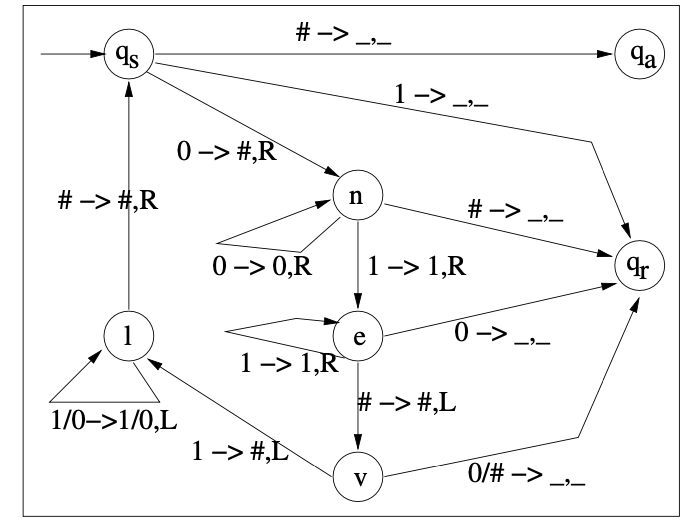
\includegraphics[scale = 0.27]{Images/TuringmachineEx.png}
    \end{minipage}
\end{theo}

% \begin{theo}[Herkennen]{Herkennen}
%     Een Turingmachine TM \textbf{herkent} een taal $L$
% \end{theo}

\begin{theo}[Turing-herkenbare taal]{Turing-herkenbare taal}
    Een taal L is \textbf{Turing-herkenbaar} als er een Turingmachine TM bestaat zodanig dat
    \begin{equation*}
        L = L_{\text{TM}}.
    \end{equation*}
    \textbf{Opmerking:} $\infty_{\text{TM}}$ is niet leeg: voor elke string niet in $L$ gaat de machine in een lus.
\end{theo}

\begin{theo}[Turing-beslisbare taal]{Turing-beslisbare taal}
    Een taal L is \textbf{Turing-beslisbaar} als er een Turingmachine TM bestaat zodanig dat
    \begin{equation*}
        L = L_{\text{TM}} \text{ en } \infty_{\text{TM}} = \emptyset.
    \end{equation*}
    \vspace{-0.3cm}
\end{theo}

\begin{theo}[Co-herkenbaar/co-beslisbaar]{Co-herkenbaar/co-beslisbaar}
    Een taal $L$ is co-herkenbaar/co-beslisbaar als $\overline{L}$ herkenbaar/beslisbaar is.
\end{theo}

\newpage

\begin{lem}[Turing-beslisbaarheid en Turing-herkenbaarheid]{Turing-beslisbaarheid en Turing-herkenbaarheid}
    \begin{enumerate}
        \item Als een taal $L$ beslisbaar is, dan is $L$ co-beslisbaar.
        \item Als een taal $L$ herkenbaar en co-herkenbaar is, dan is $L$ beslisbaar.
        \item Er bestaat een taal die niet herkenbaar is.
    \end{enumerate}
\end{lem}

\begin{prf}[Turing-beslisbaarheid en Turing-herkenbaarheid]{Turing-beslisbaarheid en Turing-herkenbaarheid}
    \begin{enumerate}
        \item 
            Verwissel de rol van $q_a$ en $q_r$ in de Turingmachine die $L$ beslist.
        \item 
            Laat $M_1$ de machine zijn die $L$ herkent, en $M_2$ de machine die $\overline{L}$ herkent. De idee is nu dat we $M_1$ en $M_2$ samen laten lopen als een nieuwe machine $M$, in parallel: zodra $M_1$ accepteert, dan accepteert $M$, en zodra $M_2$ accepteert, dan verwerpt $M$. $M_1$ en $M_2$ kunnen niet samen accepteren, en voor elke string zal minstens één van de machines $M_1$ en $M_2$ stoppen p in zijn aanvaardende toestand. $M$ beslist $L$.
        \item 
            Het bewijs steunt op het begrip kardinaliteit: we weten van vroeger dat het aantal Turingmachines aftelbaar oneindig is. We weten ook dat elke Turingmachine juist één taal herkent. En tenslotte weten we ook dat het aantal talen niet-aftelbaar oneindig is, want de verzameling talen is $\mathcal{P}(\Sigma^*)$. Bijgevolg bestaat een niet-herkenbare taal. In feite is daarmee zelfs bewezen dat er niet-aftelbaar veel niet-herkenbare talen bestaan. Meer nog: bijna alle talen zijn niet-herkenbaar!
    \end{enumerate}
\end{prf}

\subsection{Encodering}

\vspace{0.5cm}

\begin{theo}[Encodering]{Encodering}
    Een encodering is een mapping van objecten in $\Sigma$ naar strings in $\Sigma^*$. Encoderingen zijn \textbf{redelijk}:
    \begin{itemize}
        \item Elk object moet minstens 1 encodering in $\Sigma^*$ hebben.
        \item Elke encodering moet volledig het object dat het encodeert bepalen.
        \item De nodige operaties moeten berekenbaar zijn uit de encodering van de objecten.
        \item Een redelijke encodering introduceert geen extra informatie.
    \end{itemize}
\end{theo}

\begin{theo}[Universele Turingmachine]{Universele Turingmachine}
    De Universele Turingmachine kan elke TM simuleren, als die maar geëncodeerd wordt zoals nodig: we kunnen de UTM zelfs laten beginnen met controleren of wat op de banden staat wel een geldige encodering is.
\end{theo}

\subsection{Het Halting-probleem}

\vspace{0.5cm}

\begin{theo}[Acceptatieprobleem]{Acceptatieprobleem}
    Stel een Turingmachine M voor met een input $w$. De \textbf{acceptatietaal} A$_{\text{TM}}$ is 
    \begin{equation*}
        \text{A}_{\text{TM}} = \{ \langle M,s \rangle \ | \ M \text{ is een Turingmachine en } s \in L_{\text{M}} \}
    \end{equation*}
    zodanig dat de Turingmachine A de taal \textbf{beslist}. Dit is een verwant probleem aan het Halting-probleem.
    \vspace{-0.5cm}
\end{theo}

\begin{lem}[Acceptatietaal is niet beslisbaar, maar wel herkenbaar]{Acceptatietaal is niet beslisbaar, maar wel herkenbaar}
    A$_{\text{TM}}$ is niet beslisbaar, maar A$_{\text{TM}}$ is herkenbaar.
\end{lem}

\begin{prf}[Acceptatietaal is niet beslisbaar, maar wel herkenbaar]{prf - Acceptatietaal is niet beslisbaar, maar wel herkenbaar}
    \begin{itemize}
        \item 
            We bewijzen door middel van contradictie. Stel er bestaat een beslisser B voor A$_{\text{TM}}$. Dat betekent dat bij input $\langle \text{M},s \rangle$ B accepteert als M bij input $s$ stopt in $q_a$ en verwerpt als M bij input $s$ niet accepteert, dus stopt in zijn $q_r$ of loopt. We schrijven
            \begin{equation*}
                \text{B}(\langle \text{M},s \rangle) \ \text{is accept als M} \ s \ \text{accepteert en anders reject}.
            \end{equation*}
            Gebruikmakend van B kunnen we nu de contradictie machine C construeren, Deze neemt als input (de codering van) een Turingmachine M, roept B op met input $\langle \text{M}, \text{M} \rangle$, en als B accepteert dan verwerpt C en omgekeerd. Kortom, C heeft de eigenschap:
            \begin{equation*}
                \forall M \in \text{Turingmachines}: \ \text{C}(\langle \text{M} \rangle) = \text{opposite}(\text{B}(\langle \text{M}, \text{M} \rangle)).
            \end{equation*}
            Neem nu voor M hierboven C zelf, dan krijgen we:
            \begin{equation*}
                \hspace{2cm}\text{C}(\langle \text{C} \rangle) = \text{opposite}(\text{B}(\langle \text{C}, \text{C} \rangle)).
            \end{equation*}
            Er geldt nu het volgende:
            \begin{align*}
                \hspace{2cm}
                C \ \text{accepteert} \ C 
                    &\Leftrightarrow C(\langle C \rangle) = \text{accept} \\
                    &\Leftrightarrow \text{opposite}(\text{B}(\langle C, C \rangle)) = \text{reject} \\
                    &\Leftrightarrow C \ \text{verwerpt} \ C.
            \end{align*}
            Dit is een contradictie, dus B kan niet bestaan en is $A_{\text{TM}}$ niet beslisbaar.
        \item 
            De herkenner A voor A$_{\text{TM}}$ laat gewooon bij input $\langle \text{M},s \rangle$ de machine M lopen op input s: als M accepteert, dan accepteert A. Als M verwerpt of loopt, dan loopt A ook.
    \end{itemize}
    \vspace{-0.3cm}
\end{prf}

\newpage

\begin{theo}[Halting-probleem]{Halting-probleme}
    Stel een Turingmachine M voor met een input $w$. De \textbf{haltingtaal} H$_{\text{TM}}$ is 
    \begin{equation*}
        \text{H}_{\text{TM}} = \{ \langle M,s \rangle \ | \ M \text{ is een Turingmachine die stopt bij input } s \}
    \end{equation*}
    zodanig dat de Turingmachine H de taal \textbf{beslist}.
\end{theo} 

\begin{lem}[Halting-taal is niet beslisbaar, maar wel herkenbaar]{Halting-taal is niet beslisbaar, maar wel herkenbaar}
    H$_{\text{TM}}$ is niet beslisbaar, maar H$_{\text{TM}}$ is herkenbaar.
\end{lem}

\begin{prf}[Halting-taal is niet beslisbaar, maar wel herkenbaar]{prf - Halting-taal is niet beslisbaar, maar wel herkenbaar}
    \begin{itemize}
        \item 
            Stel dat H$_{\text{HM}}$ beslisbaar is door een Turingmachine H. We construeren nu beslisser B voor A$_{\text{HM}}$ als volgt: bij input $\langle \text{M} ,s \rangle$ doet B:
            \begin{itemize}
                \item laat eerst H lopen op $\langle \text{M} ,s \rangle$
                \item $H(\langle \text{M} ,s \rangle) = \text{accept} \Rightarrow$ B accepteert en geeft als resultaat wat M geeft 
                \item $H(\langle \text{M} ,s \rangle) = \text{reject} \Rightarrow$ reject B ook de string $\langle \text{M} ,s \rangle$. 
            \end{itemize}
            Vermits er geen beslisser voor A$_{\text{HM}}$ bestaat, kan H niet bestaan en is dus ook H$_{\text{HM}}$ niet beslisbaar zijn.
        \item
            De herkenner H voor H$_{\text{HM}}$ laat gewoon bij input $\langle \text{M} ,s \rangle$ de machine M lopen op input s: als M stopt, dan accepteert H. Als M loopt, dan loopt H ook.
    \end{itemize}
\end{prf}

\begin{lem}[De complemententalen zijn niet herkanbaar]{De complemententalen zijn niet herkanbaar}
    $\overline{\text{A}_{\text{TM}}}$ en $\overline{\text{H}_{\text{TM}}}$ zijn niet herkenbaar.
\end{lem}

\begin{prf}[De complemententalen zijn niet herkanbaar]{prf - De complemententalen zijn niet herkanbaar}
    \begin{itemize}
        \item 
            Als $\overline{\text{A}_{\text{TM}}}$ herkenbaar is,en vermits herkenbaar is, dan is ook $\text{A}_{\text{TM}}$ beslisbaar. Maar dat is niet het geval, dus $\overline{\text{A}_{\text{TM}}}$ is niet herkenbaar.
        \item 
            Als $\overline{\text{H}_{\text{TM}}}$ herkenbaar is,en vermits herkenbaar is, dan is ook $\text{H}_{\text{TM}}$ beslisbaar. Maar dat is niet het geval, dus $\overline{\text{H}_{\text{TM}}}$ is niet herkenbaar.
    \end{itemize}
\end{prf}